\chapter{Decomposition Approach Evaluation}
\label{appendix:decompositionAppraoches}

During early feasibility tests with graph clustering, we encountered significant problems as documented in the next Section. As consequence of these results, we conducted a feasibility assessment with a professor of mathematics on the graph based approach, documented in Appendix \ref{sec:feasibilityAssessment}. Out of the feasibility assessment, two additional approaches on how the Service Cutter can solve the decomposition problem were defined and are discussed in this Chapter. Nevertheless, the conclusion Section states how challenges in these approaches and further research on clustering graphs led us back to follow the graph based approach.

\section{Graph Clustering Problems}

At first, the clustering algorithm evaluated documented in Appendix \ref{appendix:graphClustering} did not contain the Leung algorithm as this has been found later during the project. The two candidate algorithms were MCL and Girvan-Newman. We did a feasibility test using a small Booking System sample containing three entities:

\begin{description}
	\item[Customer Entity] containing address, accountNr, creditCardNr, and name.
	\item[Article Entity] containing articleName, price, and serial.
	\item[Booking Entity] containing stotalPrice, paymentDate, bookingDate, and bookingState.
\end{description}

\begin{figure}[H]
	\begin{center}
		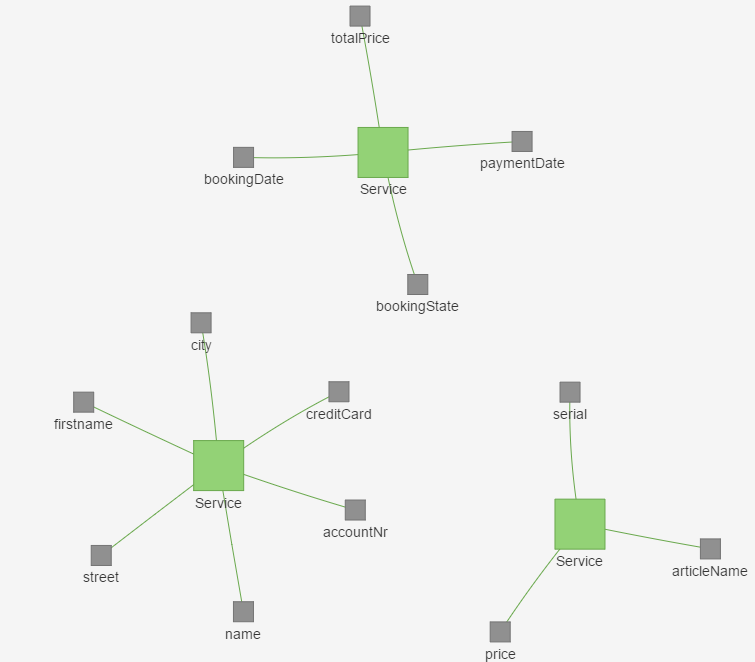
\includegraphics[scale=0.75]{images/booking_entities.png}
	\end{center}
	\caption{Expected output for Booking Example}
	\label{fig:bookingExample}
\end{figure}

To keep the sample simple we only added information for the \textit{Lifecycle \& Identity Commonality} criterion, so that the output is expected to show exactly the entity borders as shown in Figure \ref{fig:bookingExample}.


\begin{figure}[H]
	\begin{center}
		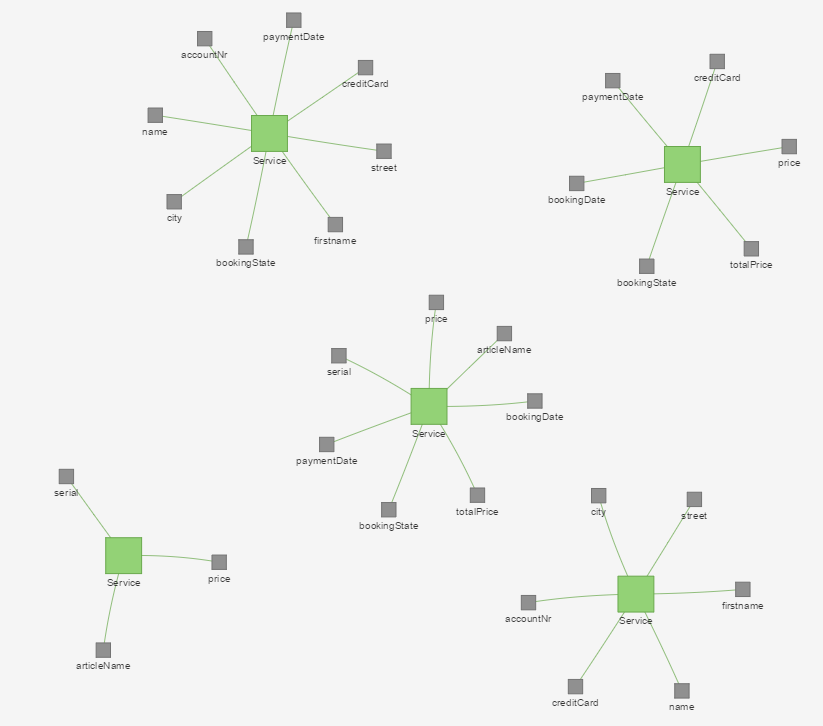
\includegraphics[scale=0.7]{images/booking_entities_mcl.png}
	\end{center}
	\caption{Booking Example with the MCL algorithm}
	\label{fig:bookingExampleMCL}
\end{figure}

The MCL algorithm's result for this example are shown in Figure \ref{fig:bookingExampleMCL}. Obviously this does not match the expectations. Nanoentities are attached to multiple services. This behavior does not meet the \textit{distinct clusters} requirement that a nanoentity should be assigned to one and only one service. 

The distinct clusters requirement is satisfied by the original MCL implementation written in R, so that the problems can be identified as implementation problem. A solution to this problem would be to write a Java wrapper for the R implementation as described in Section \ref{subsec:mclAdapter}.

\begin{figure}[H]
	\begin{center}
		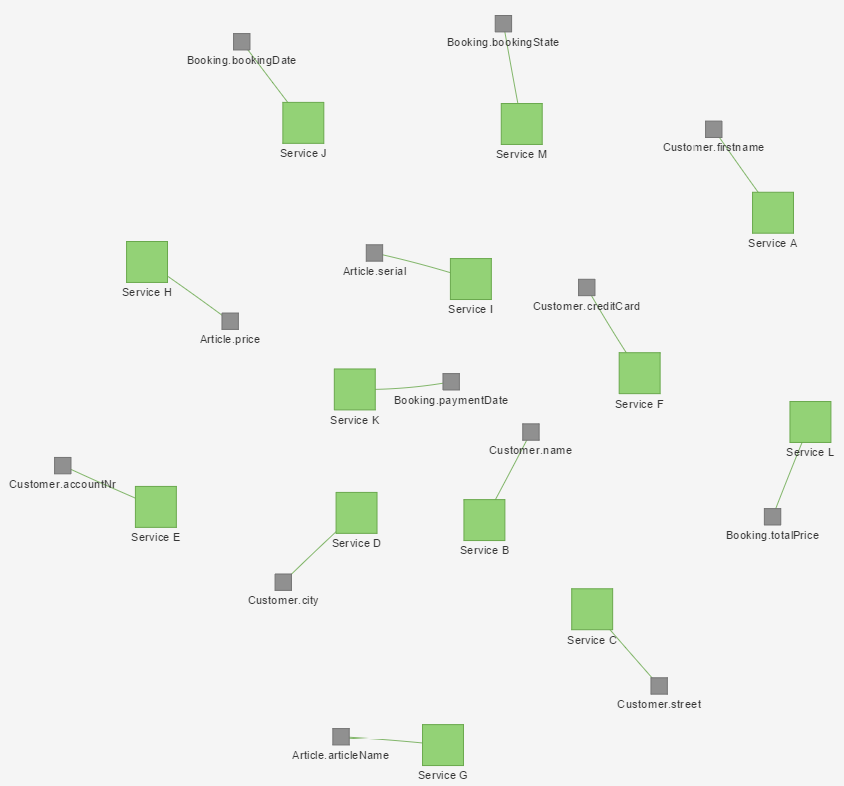
\includegraphics[scale=0.65]{images/girvan_entities_fail.png}
	\end{center}
	\caption{Booking Example with the Girven-Newman algorithm}
	\label{fig:bookingExampleGirvan}
\end{figure}

Figure \ref{fig:bookingExampleGirvan} shows the unsatisfying result provided by Girvan-Newman. By reasons of these unexpected results, we consulted a professor of mathematics as documented in Appendix \ref{sec:feasibilityAssessment} which lead to the alternative approaches described in the next Sections.

\section{Approach \#2: Rating of Possible Service Cuts}

The idea this approach introduces is to create a set of all possible service cuts and rate the cuts isolated per coupling criteria. The approach is illustrated in Figure \ref{fig:setProcess}.

%TODO update Data Fields to NanoEntities, Processor to Scorer
\begin{figure}[H]
	\begin{center}
		\includegraphics[scale=0.45]{diagrams/scoring_process.png}
	\end{center}
	\caption{Approach \#2: Set Rating}
	\label{fig:setProcess}
\end{figure}

This approach is processed in three steps:

\begin{description}
	\item[Partitioning] Based on the nanoentities, a set of all possible candidate service cuts is calculated. This includes every theoretically possible service cut for every number of services. For practical usage, this step needs to be optimized. 
	\item[Assessment] For all coupling criteria a processor assesses all service cuts with a score describing how well the criteria's requirements are met. The score is a number between 0 and 10, while 10 implies that all requirements are perfectly satisfied. 
	\item[Evaluation] The user optionally defines priorities how important each criteria is for his system. The priorities are defined with approximately exponential numbers like the Fibonacci sequence. These priorities are applied on the service cut scores. The resulting best candidate cut is then presented to the user.
\end{description}

\subsection{Discussion}

An advantage of this approach is that each relevant step is clearly separated and can thus be analyzed, debugged and visualized better than in the graph based approach. The assessment and score calculation is done separately for every cut and for every coupling criteria. Each criteria scorer scores candidate cuts with a uniform scoring range. As solutions do not need to be constructed but only rated, the single dimensionality problem described in Section \ref{subsec:singleDimensionality} does not apply.

The weak point is the partitioning process. Theoretically every possible set of services where each nanoentity is contained in one and only one service is a candidate cut. In mathematics this is described as the \textit{partition of a set}\cite{partitionOfASet} problem. The Bell number $B_n$ defines the amount of possible partitions: 


\begin{displaymath}
B_{n+1}=\sum_{j=0}^n {n\choose j} B_j
\end{displaymath}

For the Service Cutter, $n$ is the number of nanoentities. The number of possible service cuts for $n=20$ nanoentities is $51'724'158'235'372$\footnote{We do not print the number for the required $2000$ nanoentities for lack of space in this document.}.

The Bell number includes cuts for $1 - n$ number of services. In the context of a software system only certain numbers of services are realistic. The \textit{Stirling numbers of the second kind} calculate the Bell number for a given number of sets $k$:

\begin{displaymath}
\left\{ {n \atop k}\right\} = \frac{1}{k!}\sum_{j=0}^{k} (-1)^{k-j} \binom{k}{j} j^n
\end{displaymath}

For $n=20$ nanoentities and $k=4$ services the equation results in $45'232'115'901$ possible cuts. For $k=6$ the result is $4'306'078'895'384$.

During a discussion with our industry partner and supervisor documented in Appendix \ref{sec:status22102015}, we decided that the Service Cutter should be able to process system models with up to 2000 nanoentities. We therefore concluded in the same meeting that this approach is not practicable without a heuristic approach of finding a small set of relevant candidate cuts. 

A possible heuristic approach is to take into account one or a few coupling criteria information about the system to find service candidates. A simple example would be to only analyze cuts where nanoentities of the same entity are not split across services so that only entities and not it's nanoentities need to be considered.

As we tried to find a heuristic approach to calculate candidate cuts, we discovered a new idea for the composition algorithm described in the next Section. 

\section{Approach \#3: Constructing Services - a Heuristic Approach}

While analyzing the decomposition problem we realized that finding a good number of services is one of the key challenges. Cohesiveness criteria are mainly satisfied by consolidating nanoentities in one service while compatibility criteria request exactly the opposite, namely the separation of nanoentities. Figure \ref{fig:numberOfServices} illustrates this dilemma.

\begin{figure}[H]
	\begin{center}
		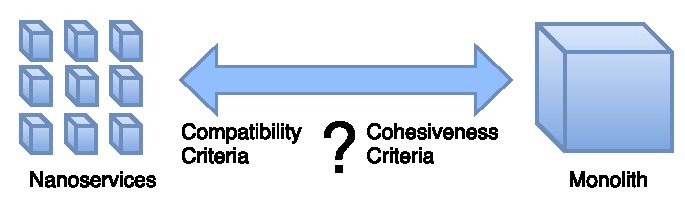
\includegraphics[scale=1]{diagrams/HeuristicApproach.pdf}
	\end{center}
	\caption{Finding a good number of services is a key challenge of service secomposition}
	\label{fig:numberOfServices}
\end{figure}

To simplify the problem for the heuristic approach we assume the number of services is given by the user and does not need to be computed. Very often an architect has a reasonable assumption about the number of services suitable for his system.

The heuristic approach starts with a unordered list of all nanoentities and services that can be imagined as empty boxes that are incrementally filled. The algorithm runs multiple iterations of construction and optimization steps.

\begin{description}
	\item[Construction] Nanoentities are sequentially taken from the list and put in the best suitable service. The target service is calculated by the criteria scores between the selected nanoentity and the nanoentities a service contains at that point of time. 
	\item[Optimization] Within a service the score from each nanoentity to all it's neighbors in the same service is calculated to determine the least suitable nanoentity in a service. This nanoentity is taken out of the service and put back on the list of unassigned nanoentities.
\end{description}

%TODO: illsutration?

The algorithm alternates between construction and optimization steps. It finishes either by a given time, by the user stopping the optimization or by detecting that no further optimization is possible. This is detected if nanoentities taken from services in the optimization step are put back to their original service during the construction step.

In an attempt to implemented this heuristic approach we realized that even if the algorithm works well, it does not accurately solve the desired problem. The approach focuses only on cohesion within services but does not take coupling between services, that should be minimized, into consideration.

While acceptable results might still be possible using this approach, we decided to focus more on graph clustering due to new findings described in the next Section.

\subsection{New Findings on Graph Clustering}

As both alternative approaches did not promise expected results, we decided to focus on further investigations on graph clustering. 

By analyzing the Girvan-Newman algorithm documented in Section \ref{subsec:girvanNewman}, we were able to identify the problem encountered with the booking sample. As the sample only provides \textit{Lifecycle \& Identity Commonality} data, every pair of nanoentities in the graph was either directly or not connected at all. The calculated edge betweenness, that Girvan-Newman is based on, is therefore equal for all edges in the graph as every shortest path only passes one edge. The Gephi\cite{gephi} implementation of Girvan-Newman consequently removes all graphs in the first iteration leaving every nanoentity isolated which results in one service per nanoentity. Adding only one more information like nanoentity characteristics or use cases solved the problem.

Through further research on the topic we found the algorithm defined by Leung implemented in the GraphStream\cite{leungGraphstream} project and integrated it into the Service Cutter. First tests using the booking sample provided the expected results.

\subsection{Conclusion}

While all approaches possibly lead to the desired results, the new findings on the Girvan-Newman and Leung algorithms promised the best results with adequate effort. Rating possible service cuts or heuristic construction of services would have both required great effort, which we decided together with our stakeholders, is not worth taking if the graph clustering provides reasonable results. 

We furthermore implemented a hint in the Service Cutter if the case arrives where a user provides input generating the faulty behavior of Girvan-Newman. %TODO implement